\section{Zielsetzung}
Laser (\textbf{l}ight \textbf{a}mplification by \textbf{s}timulated \textbf{e}mission of \textbf{r}adiation) sind in der experimentellen Physik von zentraler Bedeutung
und werden u.a. zur Untersuchung atomarer Strukturen genutzt. Sie bieten eine leistungsstarke Quelle für kohärentes Licht und sind 
oft auf bestimmte Wellenlängen einstellbar. In diesem Versuch wird die Funktionsweise eines Diodenlasers, die Justierung des Lasers
und dessen Bedienung im Experiment am Beispiel des Absorptionsspektrums von Rubidium erprobt.


\section{Theorie}
\label{sec:Theorie}

\subsection{Zustandssysteme und Besetzungsinversion}
Das Funktionsprinzip eines Lasers beruht auf der quantenmechanischen Beschreibung von Zustandssystemen. Demnach lassen sich Systeme von Teilchen (z.B. Elektronen oder Atome)
durch ein Zustandssystem beschreiben, bei dem jedem möglichen Zustand eine Energie zugeordnet wird. Damit ein Teilchen in einen energetisch höheren Zustand gelangen kann,
muss es genau die Energiedifferenz zwischen den beiden Zuständen überwinden. Dies ist über die Absorption eines Photons möglich, dessen Frequenz $\nu$ genau zur nötigen 
Energie $E = \symup{h}\nu$ korrespondiert. Ebenso wird bei einem Übergang in ein niedrigeres Niveau Energie frei, die in Form eines Photons emittiert wird. Ein solcher 
Übergang kann spontan auftreten (spontane Emission) oder durch ein Photon gleicher Frequenz angeregt werden (stimulierte/induzierte Emission). Bei stimulierter Emission
stimmt das emittierte Photon in Frequenz, Phasenlage und Polarisation mit dem anregenden Photon überein, weshalb dieser Vorgang zur Erzeugung von kohärentem Licht in einem 
Laser genutzt wird. Dazu müssen jedoch die energetisch höheren Zustände stets stärker besetzt sein, als energetisch Niedrige, damit die stimulierte Emission überwiegen kann. 
Dies wird \textit{Besetzungsinversion} genannt. Bei einem Zwei-Zustandssystem mit Energien $E_1 < E_2$ ist dies nicht möglich, da die Wahrscheinlichkeiten der Übergänge
$E_1 -> E_2$ und $E_2 -> E_1$ gleich sind und sich somit maximal eine Gleichverteilung auf die Zustände einstellen könnte. Gibt es jedoch einen weiteren Zustand zwischen
den Energieniveaus $E_1$ und $E_2$ kann Besetzungsinversion erreicht werden. Das Anregungsschema eines 4-Niveau Systems ist in \autoref{fig:4Niveau} abgebildet.
\begin{figure}
    \centering
    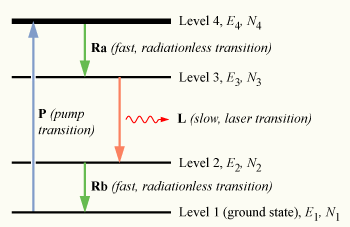
\includegraphics[scale=0.58]{content/pics/Population-inversion-4level.png}
    \caption{Anregungsschema eines 4-Niveau-Lasers. Zwischen Niveau 3 und 2 wird ein Photon durch stimulierte Emission ausgesendet. \cite{wikipedia_population_inversion}}
    \label{fig:4Niveau}
\end{figure}
Die Elektronen werden in das höchste Energieniveau \dq gepumpt\dq{} und fallen schnell in das kurz darunter liegende Niveau 3 ab. Dies geschieht mitunter sogar strahlungsfrei.
Zwischen den Niveaus 3 und 2 findet stimulierte Emission statt. Anschließend fällt das Elektron schnell und strahlungsfrei aus dem zweiten Zustand - welcher kurz über dem Ersten
liegt - in den Grundzustand zurück, aus dem es wieder in den vierten Zustand gepumpt werden kann. Durch diese Anordnung liegt immer Besetzungsinversion vor.

\subsection{Funktionsweise von Halbleiterdioden}
Eine Halbleiterdiode besteht im wesentlichen aus einem p- und einem n-dotierten Halbleitermaterial. Eine \glqq Dotierung\grqq{} meint das Einbringen von Fremdatomen in ein
Grundmaterial. Negativ geladenen Atome bringen dabei zusätzliche Elektronen in das Material, welche sich frei bewegen können. Ebenso bringen positiv geladene Atome 
\dq Fehlstellen\dq{} - auch Löcher genannt - in das Material, die sich ebenfalls frei bewegen können und sich wie positive Elektronen verhalten.
